\documentclass[11pt,a4paper]{report}

% packages
\usepackage[left=20mm, right=15mm, top=10mm, bottom=15mm]{geometry}
\usepackage{tocloft}
\usepackage{graphicx}
\usepackage{subcaption}
\usepackage{amsmath}
\usepackage{setspace}
\usepackage{makecell}
\usepackage[utf8]{inputenc}
% \usepackage{algorithmic}
\usepackage[english]{babel}
\usepackage{amsthm}
\usepackage{arevmath}     % For math symbols
\usepackage[noend]{algpseudocode}
\usepackage{amssymb}
\usepackage{algorithm2e}


\theoremstyle{definition}
\newtheorem{definition}{Definition}[section]

\theoremstyle{remark}
\newtheorem*{remark}{Remark}

\begin{document}

    \tableofcontents

    
    \section{Introduction}
    The objective of this medium-sized scientific software engineering project is to implement the power function while approaching the problem from first principles. Tasks like \textbf{documenting}, \textbf{versioning}, and \textbf{testing} are considered first class citizens.
    
    System, Software system, Eternity all refer to the same time.
    
    \chapter{Power Function}
    
        \begin{definition}
            The \textbf{power function} is defined as the function that takes any numbers $x$ and $y$ as input, raises $x$ to $y$, and returns $x^y$ as output.
        \end{definition}
    
        The power function is a transcendental function and cannot be expressed in terms of a finite sequence of the algebraic operations of raising to a power, division, multiplication, addition, subtraction, and root extraction [wikipedia].
        
        All the exponentiation rules are applicable here.
        
        \section{Domain and Co-domain} [algoritms website]
        The domains and co-domains of $x$ and $y$ vary as follows:
        
        \begin{itemize}
            \item If \textbf{base $x$ is a positive real number}, then $y$ belongs to the set of all reals numbers.
            
            The corresponding range is the set of all positive real numbers.
            
            \item If \textbf{base $x$ is zero}, then $y$ belongs to the set of non-negative real numbers.
            
            This is because a negative $y$ would lead to division by zero.
            
            \item If \textbf{base $x$ is negative}, then $y$ may only have to certain values:

                    \begin{itemize}
                        \item $y$ \textbf{may be} any integer.
                        
                        \item $y$ \textbf{may be} a fraction of the form $a/b$ where \emph{b} is odd.
                        
                        \item $y$ \textbf{may not be} a fraction of the form $a/b$ where \emph{b} is even.
                        
                        \item $y$ \textbf{may not be} an irrational number. 
                        
                    \end{itemize}
            
        \end{itemize}
        
        !!!! Please add the boundary cases here.
        
        \section{Context of use Model}
            The context of use is a description of the condtions under which the software system will be used under the normal working circumstances. 
            A context of use model is a useful tool to explore and understand the details and boundaries of a project. 
            % ["https://www.edrawmax.com/context-diagram/#:~:text=What%20are%20the%20Benefits%20of%20a%20Context%20Diagram%3F,skills%20or%20knowledge%20to%20understand%20a%20context%20diagram.]
            
            There is currently no standard for representing the context of use. A context diagram is however a suitable candidate for mind mapping. 
            
            Fig 1. is a context diagram for this project built using the [gitmind tool]. It focusses on the users of the systems and the environments where this system will be operated. The users block is subdivided into blocks representing the potential users of the system and their requirements for effective and efficient completion of thei responsibilities.
            
            The environment block explores the different system environments needed to perform different tasks. In particular, the developers, testers and, maintainer require a Technical environment. The end-user however doesn't require anything more than the general environment.
        
            \begin{figure}[htbp]
                \centering
                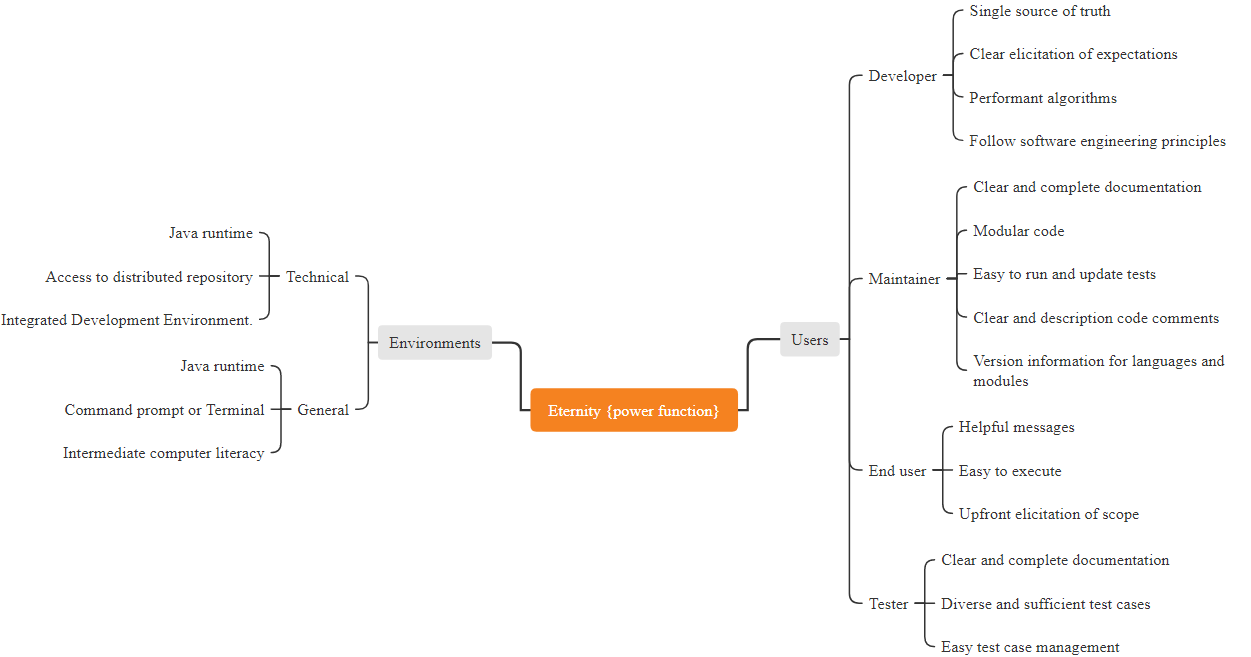
\includegraphics[width=\linewidth]{lecture-10/Context_of_use.PNG}
                \caption{Context of use for Eternity.}
                \label{fig:context_of_use}
            \end{figure}

        \chapter{Requirements}
            % This chapter lists the software requirements using the format outlined in the ISO/IEC/IEEE 29148 sections 5.2.4 to 5.2.7 (“ISO/IEC/IEEE International Standard - Systems and Software Engineering -- Life Cycle Processes -- Requirements Engineering,” 2018, #). 
            The following meta data is associated with each requirement:
        
            \begin{description}
                \item[ID] This string uniquely identifies the requirement.
                \item[VERSION] This indicates the number of times a requirement has been updated.
                \item[PRIORITY] This string indicates the importance of implementing this requirement for the minimum viable product. Priority may be one of HIGH, AVERAGE, or LOW.
                \item[TYPE] This string indicates whether the requirement is functional or non-functional in nature.        
            \end{description}
            \vspace{3em}

        % Tables for requirements.
        % Requirement 1
        \begin{table}[ht]
            \centering
                \begin{tabular}{cccc} % ll can be replace with c. | is a table line
                    \textbf{ID} & \textbf{VERSION} & \textbf{PRIORITY} & \textbf{TYPE}\\
                            R1  &           1      &           HIGH    &      NON-FUNCTIONAL\\
                    \hline
                    \multicolumn{4}{l}{Eternity shall execute on any device with JVM.}
                \end{tabular}
                \caption{Requirement 1}
                \label{tab:table-requirements-1}
            \end{table}
            \vspace{3em}
            
            % Requirement 2
            \begin{table}[ht]
            \centering
                \begin{tabular}{cccc} % ll can be replace with c. | is a table line
                    \textbf{ID} & \textbf{VERSION} & \textbf{PRIORITY} & \textbf{TYPE}\\
                            R2  &           1      &           HIGH    &      FUNCTIONAL\\
                    \hline
                    \multicolumn{4}{l}{Eternity shall allow multiple calculations per session}
                \end{tabular}
                \caption{Requirement 2}
                \label{tab:table-requirements-2}
            \end{table}
            \vspace{3em}
            
            % Requirement 3
            \begin{table}[ht]
            \centering
                \begin{tabular}{cccc} % ll can be replace with c. | is a table line
                    \textbf{ID} & \textbf{VERSION} & \textbf{PRIORITY} & \textbf{TYPE}\\
                            R3  &           1      &           HIGH    &      NON-FUNCTIONAL\\
                    \hline
                    \multicolumn{4}{l}{Eternity shall be developed with maintainability in mind.}
                \end{tabular}
                \caption{Requirement 3}
                \label{tab:table-requirements-3}
            \end{table}
            \vspace{3em}
    
            % Requirement 4
            \begin{table}[ht]
            \centering
                \begin{tabular}{cccc} % ll can be replace with c. | is a table line
                    \textbf{ID} & \textbf{VERSION} & \textbf{PRIORITY} & \textbf{TYPE}\\
                            R4  &           1      &           HIGH    &      NON-FUNCTIONAL\\
                    \hline
                    \multicolumn{4}{l}{Eternity shall be modular and testable.}
                \end{tabular}
                \caption{Requirement 4}
                \label{tab:table-requirements-4}
            \end{table}
            \vspace{3em}

        % Requirement 5
        \begin{table}[ht]
            \centering
                \begin{tabular}{cccc} % ll can be replace with c. | is a table line
                    \textbf{ID} & \textbf{VERSION} & \textbf{PRIORITY} & \textbf{TYPE}\\
                            R5  &           1      &           HIGH    &      NON-FUNCTIONAL\\
                    \hline
                    \multicolumn{4}{l}{Eternity shall have a simple user interface to increase usability.}
                \end{tabular}
                \caption{Requirement 5}
                \label{tab:table-requirements-5}
            \end{table}
            \vspace{3em}
            
            % Requirement 6
            \begin{table}[ht]
            \centering
                \begin{tabular}{cccc} % ll can be replace with c. | is a table line
                    \textbf{ID} & \textbf{VERSION} & \textbf{PRIORITY} & \textbf{TYPE}\\
                            R6  &           1      &           HIGH    &      FUNCTIONAL\\
                    \hline
                    \multicolumn{4}{l}{Eternity shall allow only integer values of $y$ when calculating $x^y$.}
                \end{tabular}
                \caption{Requirement 6}
                \label{tab:table-requirements-6}
            \end{table}
            \vspace{3em}
            
            % Requirement 7
            \begin{table}[ht]
            \centering
                \begin{tabular}{cccc} % ll can be replace with c. | is a table line
                    \textbf{ID} & \textbf{VERSION} & \textbf{PRIORITY} & \textbf{TYPE}\\
                            R7  &           1      &           HIGH    &      FUNCTIONAL\\
                    \hline
                    \multicolumn{4}{l}{Eternity shall allow all real values for $x$ when calculating $x^y$.}
                \end{tabular}
                \caption{Requirement 7}
                \label{tab:table-requirements-7}
            \end{table}
            \vspace{3em}
            
            % Requirement 8
            \begin{table}[ht]
            \centering
                \begin{tabular}{cccc} % ll can be replace with c. | is a table line
                    \textbf{ID} & \textbf{VERSION} & \textbf{PRIORITY} & \textbf{TYPE}\\
                            R8  &           1      &           HIGH    &      NON-FUNCTIONAL\\
                    \hline
                    \multicolumn{4}{l}{Eternity shall provide a help menu for users.}
                \end{tabular}
                \caption{Requirement 8}
                \label{tab:table-requirements-8}
            \end{table}
            \vspace{3em}
            
            % Requirement 9
            \begin{table}[ht]
            \centering
                \begin{tabular}{cccc} % ll can be replace with c. | is a table line
                    \textbf{ID} & \textbf{VERSION} & \textbf{PRIORITY} & \textbf{TYPE}\\
                            R9  &           1      &           HIGH    &      NON-FUNCTIONAL\\
                    \hline
                    \multicolumn{4}{l}{Eternity shall provide Javadoc documentation.}
                \end{tabular}
                \caption{Requirement 9}
                \label{tab:table-requirements-9}
            \end{table}
            \vspace{3em}
            
            % Requirement 10
            \begin{table}[ht]
            \centering
                \begin{tabular}{cccc} % ll can be replace with c. | is a table line
                    \textbf{ID} & \textbf{VERSION} & \textbf{PRIORITY} & \textbf{TYPE}\\
                            R10  &           1      &           HIGH    &      FUNCTIONAL\\
                    \hline
                    \multicolumn{4}{l}{Eternity shall use optimal algorithms.}
                \end{tabular}
                \caption{Requirement 10}
                \label{tab:table-requirements-10}
            \end{table}
            \vspace{3em}
            
            % Requirement 11
            \begin{table}[ht]
            \centering
                \begin{tabular}{cccc} % ll can be replace with c. | is a table line
                    \textbf{ID} & \textbf{VERSION} & \textbf{PRIORITY} & \textbf{TYPE}\\
                            R11  &           1      &           HIGH    &      FUNCTIONAL\\
                    \hline
                    \multicolumn{4}{l}{Eternity shall not allow $x$ to be 0 when $y$ is negative.}
                \end{tabular}
                \caption{Requirement 11}
                \label{tab:table-requirements-11}
            \end{table}
            \vspace{3em}
            
            % Requirement 12
            \begin{table}[ht]
            \centering
                \begin{tabular}{cccc} % ll can be replace with c. | is a table line
                    \textbf{ID} & \textbf{VERSION} & \textbf{PRIORITY} & \textbf{TYPE}\\
                            R12  &           1      &           HIGH    &      FUNCTIONAL\\
                    \hline
                    \multicolumn{4}{l}{Eternity shall return 1 when the power is 0.}
                \end{tabular}
                \caption{Requirement 12}
                \label{tab:table-requirements-12}
            \end{table}
            \vspace{3em}
            
            % Requirement 13
            \begin{table}[ht]
            \centering
                \begin{tabular}{cccc} % ll can be replace with c. | is a table line
                    \textbf{ID} & \textbf{VERSION} & \textbf{PRIORITY} & \textbf{TYPE}\\
                            R13  &           1      &           HIGH    &      FUNCTIONAL\\
                    \hline
                    \multicolumn{4}{l}{Eternity shall return $x$ when $y$ = 1 in $x^y$.}
                \end{tabular}
                \caption{Requirement 13}
                \label{tab:table-requirements-13}
            \end{table}
            \vspace{3em}
            
            % Requirement 14
            \begin{table}[ht]
            \centering
                \begin{tabular}{cccc} % ll can be replace with c. | is a table line
                    \textbf{ID} & \textbf{VERSION} & \textbf{PRIORITY} & \textbf{TYPE}\\
                            R14  &           1      &           LOW    &      FUNCTIONAL\\
                    \hline
                    \multicolumn{4}{l}{Eternity will maintain a history of previous operations.}
                \end{tabular}
                \caption{Requirement 14}
                \label{tab:table-requirements-14}
            \end{table}
            \vspace{3em}

    \chapter{Algorithm}
            There exist a few algorithms for calculating the power function. However, requirements \ref{tab:table-requirements-6} and \ref{tab:table-requirements-7} significantly reduce the scope this project.
            We will consider two algorithms for Eternity, the repeated multiplication or iterative solution and, the divide and conquer solution.
            When discussing these algorithms we will assume that the power $y$ is positive since the solution for negative $y$ can be derived trivially from this value.

            \section{Iterative Solution $\langle$ Naive approach $\rangle$} % algorithm level
        	The iterative solution is the simplest way solve this problem. The calculation of $x^y$ involves multiplying \emph{X} with itself exactly $y$ times.
        	For example, $2^3 \, = \, 2 \, * \, 2 \, * \, 2 \, = \, 8$.
        	
        	\subsection{Pseudocode}
        % 	\begin{verbatim}
        % 	    power = 1
        % 	    while y > 0:
        % 	        power = power * x
        % 	        y = y - 1
        % 	    print (power)
        % 	\end{verbatim}
        	
            % 	\begin{algorithmic}
            % 	    \STATE {$power \gets 1$}
            % 	    \WHILE {$y > 0$}
            % 	        \STATE {$power \gets power * x$}
            % 	        \STATE {$y = y - 1$}
            % 	    \ENDWHILE
            % 	    \RETURN {$power$}
            % 	\end{algorithmic}
            	\begin{description}
                	\item [Input]: Numbers $x$ and $y$ where $x$ is a real number and $y$ is a positive integer.
                	\item [Output]: Return the value power function $x^y$.
            	\end{description}
            	
            	\begin{algorithm}
                	\SetKwInput{function}{Function}
                	\function{$power\_incremental$($x, y$)}
                	    $power \gets 1$\;
                	    \While{$y > 0$}{
                	        $power \gets power * x$\;
                	        $y = y - 1$\;
                	    }
                	    \Return {$power$}\;
                \caption{Power function using repeated multiplication (Naive).}
                \label{alg:power-incremental}
            	\end{algorithm}
            	
            \subsection{Complexity}
            This is a relatively straightforward algorithm and runs in linear time. This results to a time complexity of $O(n)$ where $n$ is the magnitude of power $y$.
        
        \clearpage

        \section{Divide and Conquer}
        In the \textbf{Divide and Conquer} approach the problem is defined recursively as follows:
            $$power(x, \, y) = power(x, \, y \, / \, 2) \, * \, power(x, \, y \, / \, 2), \, if \, y \, is \, even$$
            $$power(x, \, y) = x \, * \, power(x, \, y \, / \, 2) \, * \, power(x, \, y \, / \, 2), \, if \, y \, is \, odd$$
        
        Here, the problem is being divided into a sub-problem which is half the size of the original problem until the base case is reached where $y \, = \, 1.$
        
            \subsection{Pseudocode}
            	\begin{description}
                	\item [Input]: Numbers $x$ and $y$ where $x$ is a real number and $y$ is a positive integer.
                	\item [Output]: Return the value power function $x^y$.
            	\end{description}
            	
            	\begin{algorithm}
                	\SetKwInput{function}{Function}
                	\function{$power\_divide\_and\_conquer$($x, y$)}
                        \If{$n = 0$}{
                            \Return {1}\;
                        }
                        
                        $pow \gets power\_divide\_and\_conquer(x, y / 2)$\;
                        
                        \If{$n$ is odd}{
                            \Return {$x\,*\, pow \,*\, pow$}\;
                        }{
                            \Return {$pow\,*\,pow$}\;
                        }
                \caption{Power function using divide and conquer.}
                \label{alg:power-divide-and-conquer}
            	\end{algorithm}
            
            \subsection{Complexity}
            Since this algorithm continuously divides the problem in half we get the time complexity of $\mathcal{O}(\log n)$ where $n$ is the magnitude of $y$.
\end{document}